\documentclass[border=10pt, sans]{standalone}

\usepackage{tikz}
\usetikzlibrary{intersections}
\usetikzlibrary{calc,patterns,angles,quotes}
\usetikzlibrary{arrows,calc,decorations.markings}
\usetikzlibrary{arrows}
\usetikzlibrary{plotmarks}

\usepackage{tkz-euclide}
\usepackage{tikz-dimline}
\usepackage{fontawesome}

\tikzset{every picture/.style={/utils/exec={\large\bfseries\sffamily}}}
\begin{document}
	
	\pgfarrowsdeclarecombine{|<}{>|}{|}{|}{latex}{latex}
	\def\Dimline[#1][#2][#3]{
		\begin{scope}[>=latex] % redef arrow for dimension lines
			\draw[|-|,
line width=1.1,
			decoration={markings, % switch on markings
				mark=at position .5 with {\node at (0,0.25) {#3};},
			},
			postaction=decorate] #1 -- #2 ;
		\end{scope}
	}

  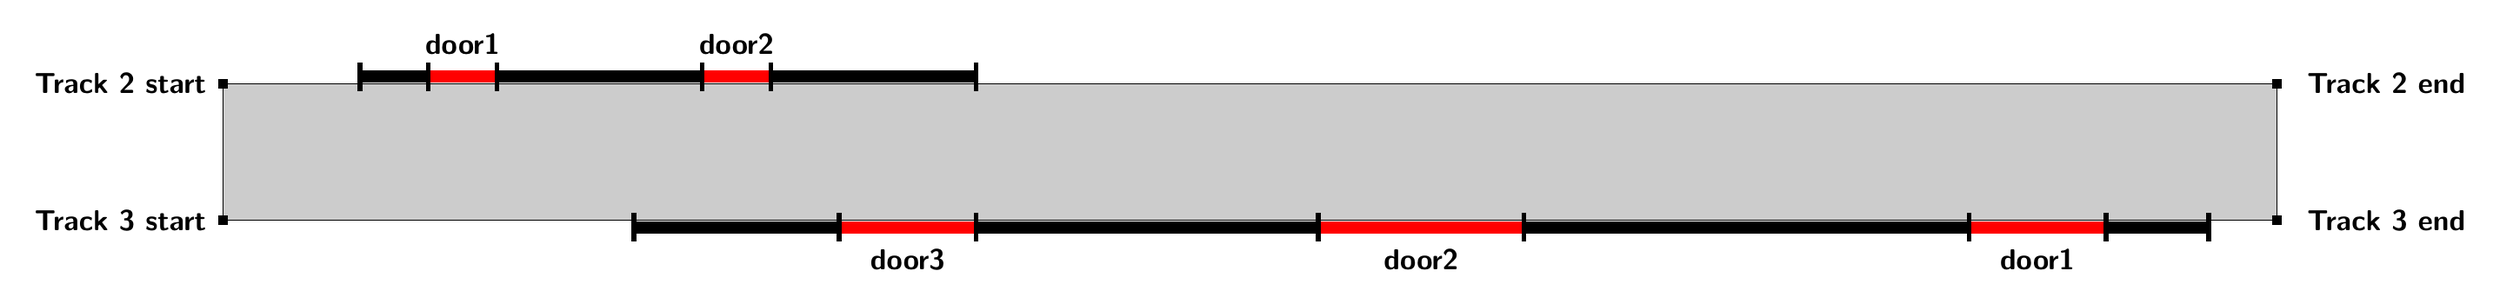
\begin{tikzpicture}[scale=1]	
  	% draw platform
  	\node (platform1) at (0, 1) {};
  	\node (platform2) at (30, -1) {};
 	\draw [fill=gray!40] (platform1.center) rectangle (platform2.center);
  
  	% draw train 1
	\def\trainOffsetOne{2}
  	\node(train1Start) at (0+\trainOffsetOne, 1.1) {};
	\node(train1Door11) at (1+\trainOffsetOne, 1.1) {};
	\node(train1Door12) at (2+\trainOffsetOne, 1.1) {};
	\node(train1Door21) at (5+\trainOffsetOne, 1.1) {};
	\node(train1Door22) at (6+\trainOffsetOne, 1.1) {};
	\node(train1End) at (9+\trainOffsetOne, 1.1) {};
	
	\draw[line width=5](train1Start.center) -- (train1End.center);
	\draw[line width=5, red](train1Door11.center) -- (train1Door12.center);
	\draw[line width=5, red](train1Door21.center) -- (train1Door22.center);
	
	\draw[line width=2, mark size=6pt]plot[mark=|] coordinates{(train1Start.center)}{};
	\draw[line width=2, mark size=6pt]plot[mark=|] coordinates{(train1Door11.center)}{};
	\draw[line width=2, mark size=6pt]plot[mark=|] coordinates{(train1Door12.center)}{};
	\draw[line width=2, mark size=6pt]plot[mark=|] coordinates{(train1Door21.center)}{};
	\draw[line width=2, mark size=6pt]plot[mark=|] coordinates{(train1Door22.center)}{};
	\draw[line width=2, mark size=6pt]plot[mark=|] coordinates{(train1End.center)}{};
	
	\node [fill=black, inner sep=2pt] (track3start) at (0, 1) {};
	\node[text width=5.5cm] at (track3start.center) 
		{Track 2 start	};
	\node [fill=black, inner sep=2pt] (track3end) at (30, 1) {};
	\node[align=right, text width=5.5cm] at (track3end.center) 
		{Track 2 end};
	\node[label=above:{door1}] at ($(train1Door11)!0.5!(train1Door12)$){};
	\node[label=above:{door2}] at ($(train1Door21)!0.5!(train1Door22)$){};
	
  	% draw train 2
	\def\trainOffsetTwo{-1}
	\node(train2Start) at (30+\trainOffsetTwo, -1.1) {};
	\node(train2Door11) at (28.5+\trainOffsetTwo, -1.1) {};
	\node(train2Door12) at (26.5+\trainOffsetTwo, -1.1) {};
	\node(train2Door21) at (20+\trainOffsetTwo, -1.1) {};
	\node(train2Door22) at (17+\trainOffsetTwo, -1.1) {};
	\node(train2Door31) at (12+\trainOffsetTwo, -1.1) {};
	\node(train2Door32) at (10+\trainOffsetTwo, -1.1) {};
	\node(train2End) at (7+\trainOffsetTwo, -1.1) {};
	
	\draw[line width=5](train2Start.center) -- (train2End.center);
	\draw[line width=5, red](train2Door11.center) -- (train2Door12.center);
	\draw[line width=5, red](train2Door21.center) -- (train2Door22.center);
	\draw[line width=5, red](train2Door31.center) -- (train2Door32.center);
	
	\draw[line width=2, mark size=6pt]plot[mark=|] coordinates{(train2Start.center)}{};
	\draw[line width=2, mark size=6pt]plot[mark=|] coordinates{(train2Door11.center)}{};
	\draw[line width=2, mark size=6pt]plot[mark=|] coordinates{(train2Door12.center)}{};
	\draw[line width=2, mark size=6pt]plot[mark=|] coordinates{(train2Door21.center)}{};
	\draw[line width=2, mark size=6pt]plot[mark=|] coordinates{(train2Door22.center)}{};
	\draw[line width=2, mark size=6pt]plot[mark=|] coordinates{(train2Door31.center)}{};
	\draw[line width=2, mark size=6pt]plot[mark=|] coordinates{(train2Door32.center)}{};
	\draw[line width=2, mark size=6pt]plot[mark=|] coordinates{(train2End.center)}{};

	\node [fill=black, inner sep=2pt] (track3start) at (0, -1) {};
	\node[text width=5.5cm] at (track3start.center) 
		{Track 3 start};
	\node [fill=black, inner sep=2pt] (track3end) at (30, -1) {};
	\node[align=right, text width=5.5cm] at (track3end.center) 
		{Track 3 end};
	\node[label=below:{door1}] at ($(train2Door11)!0.5!(train2Door12)$){};
	\node[label=below:{door2}] at ($(train2Door21)!0.5!(train2Door22)$){};
	\node[label=below:{door3}] at ($(train2Door31)!0.5!(train2Door32)$){};
	
%	% Draw dimlines
	\Dimline[(0,2)][(0+\trainOffsetOne, 2.)][offset];
	\Dimline[(0+\trainOffsetOne,2)][(9+\trainOffsetOne, 2.)][RE];
	\Dimline[(30,-2)][(30+\trainOffsetTwo, -2.)][offset];
	\Dimline[(30+\trainOffsetTwo,-2)][(7+\trainOffsetTwo, -2.)][ICE];
  \end{tikzpicture}
\end{document}